\chapter{Funktionalität}
SetlCup ist ein LR-Parser-Generator, welcher angelehnt an den bereits vorhandenen JavaCup ist.
Dabei ist die Idee wie folgt:
Der Benutzer von SetlCup erstellt durch eine gegebene Scanner- und Parserdefinition eine neue Setlx-Datei. Diese beinhaltet einen kanonischen LR-Parser, welcher auf den gegebenen Definitionen beruht. Anschließend kann eine Eingabedatei von dem generierten Parser überprüft werden. Dabei wird ggf. angegebener Code bei der Reduzierung der entsprechenden Regeln durchgeführt. 

Zunächst wird erklärt, wie die Komponente aufgerufen werden kann.
\chapter{Aufrufsmethoden}
Es gibt mehrere Möglichkeiten SetlCup aufzurufen:
\section{Aufruf über Kommandozeile}
\begin{enumerate}
	\item \begin{Verbatim}
	setlx setlcup.stlx -p parser_scanner_datei.stlx
	\end{Verbatim}
			Mit diesem Aufruf wird ein Parser gemäß der in der Eingabedatei gegebenen Definitionen erstellt.
	\item \begin{Verbatim}
	setlx setlcup.stlx -p parser_scanner_datei.stlx -d
	\end{Verbatim}
			Um die Art und Weise, wie der Parser generiert wird Nachzuvollziehen, kann mit der Option "`-d"' das Debugging eingeschaltet werden. Dabei wird empfohlen die Ausgabe in eine Datei umzuleiten.
	\item \begin{Verbatim}
	setlx parser_datei.stlx -p eingabe_datei.txt
	\end{Verbatim}
	Der erstellte Parser kann mit dem o.g. Befehl aufgerufen werden und probiert die Eingabedatei nach den angegebenen Regeln zu überprüfen.
		\item \begin{Verbatim}
	setlx parser_datei.stlx -p eingabe_datei.txt -d
	\end{Verbatim}
	Analog zur Parsererstellung wird durch die Option "`-d"' das Debugging eingeschaltet.
	\item \begin{Verbatim}
	setlx setlcup.stlx -h
	\end{Verbatim}
			Dieser Aufruf zeigt die Hilfe an, wie SetlCup aufgerufen werden kann.
\end{enumerate}
%\subsection{Calling via Setlx}
%SetlCup can also be called in Setlx itself. If this case is used, you need to load the program "setlcup\_load.stlx".
%\begin{figure}[!ht]
%\begin{Verbatim}[ frame         = lines, 
                  %framesep      = 0.3cm, 
                  %labelposition = bottomline,
                  %numbers       = left,
                  %numbersep     = -0.2cm,
                  %xleftmargin   = 0.8cm,
                  %xrightmargin  = 0.8cm,
                %]
	%load("setlcup_load.stlx");
%\end{Verbatim}
%\end{figure}
%Afterwards Setlcup can be used via the method call
%\begin{Verbatim}
	%call_generate_ast(input_grammar, file_to_parse, silent_mode);
%\end{Verbatim}
%
%e.g.
%\begin{figure}[!ht]
%\begin{Verbatim}
	%load("setlcup_load.stlx");
	%print(call_generate_ast('examples\math_expression_grammar_ast.g', 
	                    %'examples\math_expression_input.txt', true));
%\end{Verbatim}
%\end{figure}
\chapter{Aufbau der Definitionen}

Der Aufbau der Scanner- und Parserdefinitionen ist in drei Abschnitte zu unterteilen:
\begin{enumerate}
	\item Kommentare
	\item Scannerdefinition
	\item Parserdefinition
\end{enumerate}
\section{Kommentare}
Im obersten Bereich der Datei ist es möglich die Idee des Parsers zu beschreiben.
Dieser Abschnitt endet mit dem Symbol "`\%\%\%"'. 
\section{Scannerdefinition}
Der Scanner ist verantwortlich um zu Überprüfen, ob die Eingabedatei aus den angegebenen Tokens besteht. Die Syntax\mRefFigure{fig:scanner_def} wird im Folgenden erklärt.
\begin{figure}[!ht]
\begin{Verbatim}[ frame         = lines, 
                  framesep      = 0.3cm, 
                  labelposition = bottomline,
                  numbers       = left,
                  numbersep     = -0.2cm,
                  xleftmargin   = 0.8cm,
                  xrightmargin  = 0.8cm,
                ]
	INTEGER       := 0|[1-9][0-9]*     ;
	ASTERISK      := \*                ;
	WHITESPACE    := [ \t\v\r\s]       ;
	SKIP          := {WHITESPACE} | \n ;
\end{Verbatim}
\caption{Scanner Definition}
\label{fig:scanner_def}
\end{figure}
\begin{itemize}
	\item In Zeile 1 wird der Token "INTEGER" definiert. Tokens werden auf die folgende Weise deklariert:\\
					token\_name := regex ; \\
					Dabei ist folgendes bei der Syntax des regulären Ausdrucks zu beachten:
					\begin{itemize}
						\item Die Rückgabe der Capture-Gruppen z.B. "`ab\textbf{(.*)}ab"'	werden nicht unterstützt. Jedoch sind Nicht-Captures möglich: "`ab(\textbf{?:}.*)ab"'
						\item Die Nutzung der geschweiften Klammer wurde überlagert, sodass die regulären Ausdrücke der großgeschriebene Wörter innerhalb der Klammern im Nachhinein ersetz werden. Siehe Zeile 4 - "`\{TOKENNAME\}"'.
						\item Ansonsten sind die bereits in SetlX vorhandenen Regex-Ausdrücke benutzbar.
					\end{itemize}
	\item Wie in SetlX (siehe Zeile 2 und 3) müssen auch in SetlCup vordefinierte Symbole wie "$*,+,?,|,\{,\},(,),\cdots$" escaped werden .
	\item In Zeile 4 wird "SKIP"-Token genutzt. In manchen Fällen werden gewisse Tokens nicht benötigt. Diese können mithilfe des "`SKIP"'-Tokens ignoriert werden. Dabei ist die Eingabe mit der o.g. Ersetzstrategie ( "` \{TOKENNAME\}"') oder die Nutzung eines regulären Ausdrucks möglich. Verschiedene Tokens müssen mit der Pipe "`|"' separiert werden.
\end{itemize}

\section{Parserdefinition}
Die Definition der Grammatik für den Parser benutzt Konzepte aus JavaCup und ANTLR \mRefFigure{fig:example_grammer}.
\begin{figure}[!ht]
\begin{Verbatim}[ frame         = lines, 
                  framesep      = 0.3cm, 
                  labelposition = bottomline,
                  numbers       = left,
                  numbersep     = -0.2cm,
                  xleftmargin   = 0.8cm,
                  xrightmargin  = 0.8cm,
                ]
	grammar := rule_definition definition_list;
	rule_definition := rule_head '::=' body_list ';' ;
	body_list := body body_list
						| ;
	body := element_list;
  element_list := element element_list
              | ;
  element := token id;
  token := '''regex''' 
         | token_name id
         | rule_name id
         ;
  id := id_name
      |;
	expr ::= 
	  expr:e MINUS prod:p {: result := Minus(e,p);:} 
	| expr:e '+' prod:p   {: result := Plus(e,p); :} 
	| 										{: :}
	;
\end{Verbatim}
\caption{Example grammar rule}
\label{fig:example_grammer}
\end{figure}
\begin{itemize}
	\item[rule\_head] The rule\_head is the name of the rule i.e. "expr". It is possible to reference defined rules via their rule\_name
	\item[body\_list] The rule can consist of multiple bodys.
	\item[rule\_body] The body can contain multiple elements. 
	\item[rule\_element] A rule element is either a :
	\begin{enumerate}
		\item Token (defined in the scanner) e.g. "MINUS"
		\item Token in  ' ' e.g. '+' as a literal
		\item other rule\_heads e.g. "prod"
	\end{enumerate}
	The Tokens defined in the scanner, as well as the rule\_heads can have an id. This can be used in the action\_code.
	\item[action\_code] The action\_code is an optional part in a body. It needs to be at the end of the body it self. Each rule\_element can have an action\_code. In this action\_code Setlx Code can be written. By using the variable "result" it is possible to pass values between rules. The id of the elements in the respective rule can be referred to by using its name.
	\item[|] The pipe separates the different bodies.
\end{itemize}
\newpage
\section{Example}
The first example shows a simple arithmetic grammar.
The second example shows how a simple programming language can be parsed using SetlCup.
\subsection{Arithmetic grammar}
The arithmetic grammar and scanner \mRefFigure{fig:example_arithmetic_grammer} can be defined using the syntax mentioned above.
\begin{figure}[!ht]
\begin{Verbatim}[ frame         = lines, 
                  framesep      = 0.3cm, 
                  labelposition = bottomline,
                  numbers       = left,
                  numbersep     = -0.2cm,
                  xleftmargin   = 0.8cm,
                  xrightmargin  = 0.8cm,
                ]
  %%%

  INTEGER       := 0|[1-9][0-9]* ;
  WHITESPACE    := [ \t\v\r\s] ;
  SKIP          := {WHITESPACE} | \n ;

  %%%
  arith_expr 
   ::= expr_list:esl                {: result := ExprList(esl); :};

  expr_list 
   ::= expr_part:part expr_list:l {: result := [part] + l; :} 
     |                            {: result := []; :}
     ;
  expr_part 
   ::= expr:e ';'            {: result := e; :} ;
  expr 
   ::=  expr:e '+'  prod:p   {: result := Plus(e , p);  :} 
     |  expr:e '-'  prod:p   {: result := Minus(e , p); :} 
     |  prod:p               {: result := p;     :}
     ;
  prod 
   ::=  prod:p '*'  fact:f   {: result := Times(p , f); :}
     |  prod:p DIVIDE fact:f {: result := Div(p , f); :} 
     |  prod:p '%'    fact:f {: result := Mod(p , f); :} 
     |  fact:f               {: result := f;     :}
     ;
  fact 
   ::=  '(' expr:e_part ')'   {: result :=  e_part ;   :} 
     |  INTEGER:n             {: result := Integer(eval(n)); :} 
     ;
\end{Verbatim}
\caption{Example arithmetic grammar}
\label{fig:example_arithmetic_grammer}
\end{figure}
%\lstinputlisting[frame=single,numbers=left,basicstyle=\footnotesize]{math_expression_grammar_ast.g}
The input file consists of multiple lines with arithmetic expressions \ref{fig:example_arithmetic_input}.
\begin{figure}[!ht]
\begin{Verbatim}[ frame         = lines, 
                  framesep      = 0.3cm, 
                  labelposition = bottomline,
                  numbers       = left,
                  numbersep     = -0.2cm,
                  xleftmargin   = 0.8cm,
                  xrightmargin  = 0.8cm,
                ]
  1 + 2 * 3 - 4;
  1 + 2 + 3 + 4;
  1 + ( 2 * 3 ) * 5 % 6;
\end{Verbatim}
\caption{Example arithmetic input}
\label{fig:example_arithmetic_input}
\end{figure}
%\lstinputlisting[frame=single,numbers=left,basicstyle=\footnotesize]{math_expression_input.txt}
The output AST\mRefFigure{fig:arith_expr_tree} consists of the three expressions noted above.
%\lstinputlisting[basicstyle=\footnotesize,breaklines=true]{math_expression_output.txt}

\begin{figure}[!ht]
	\centering
		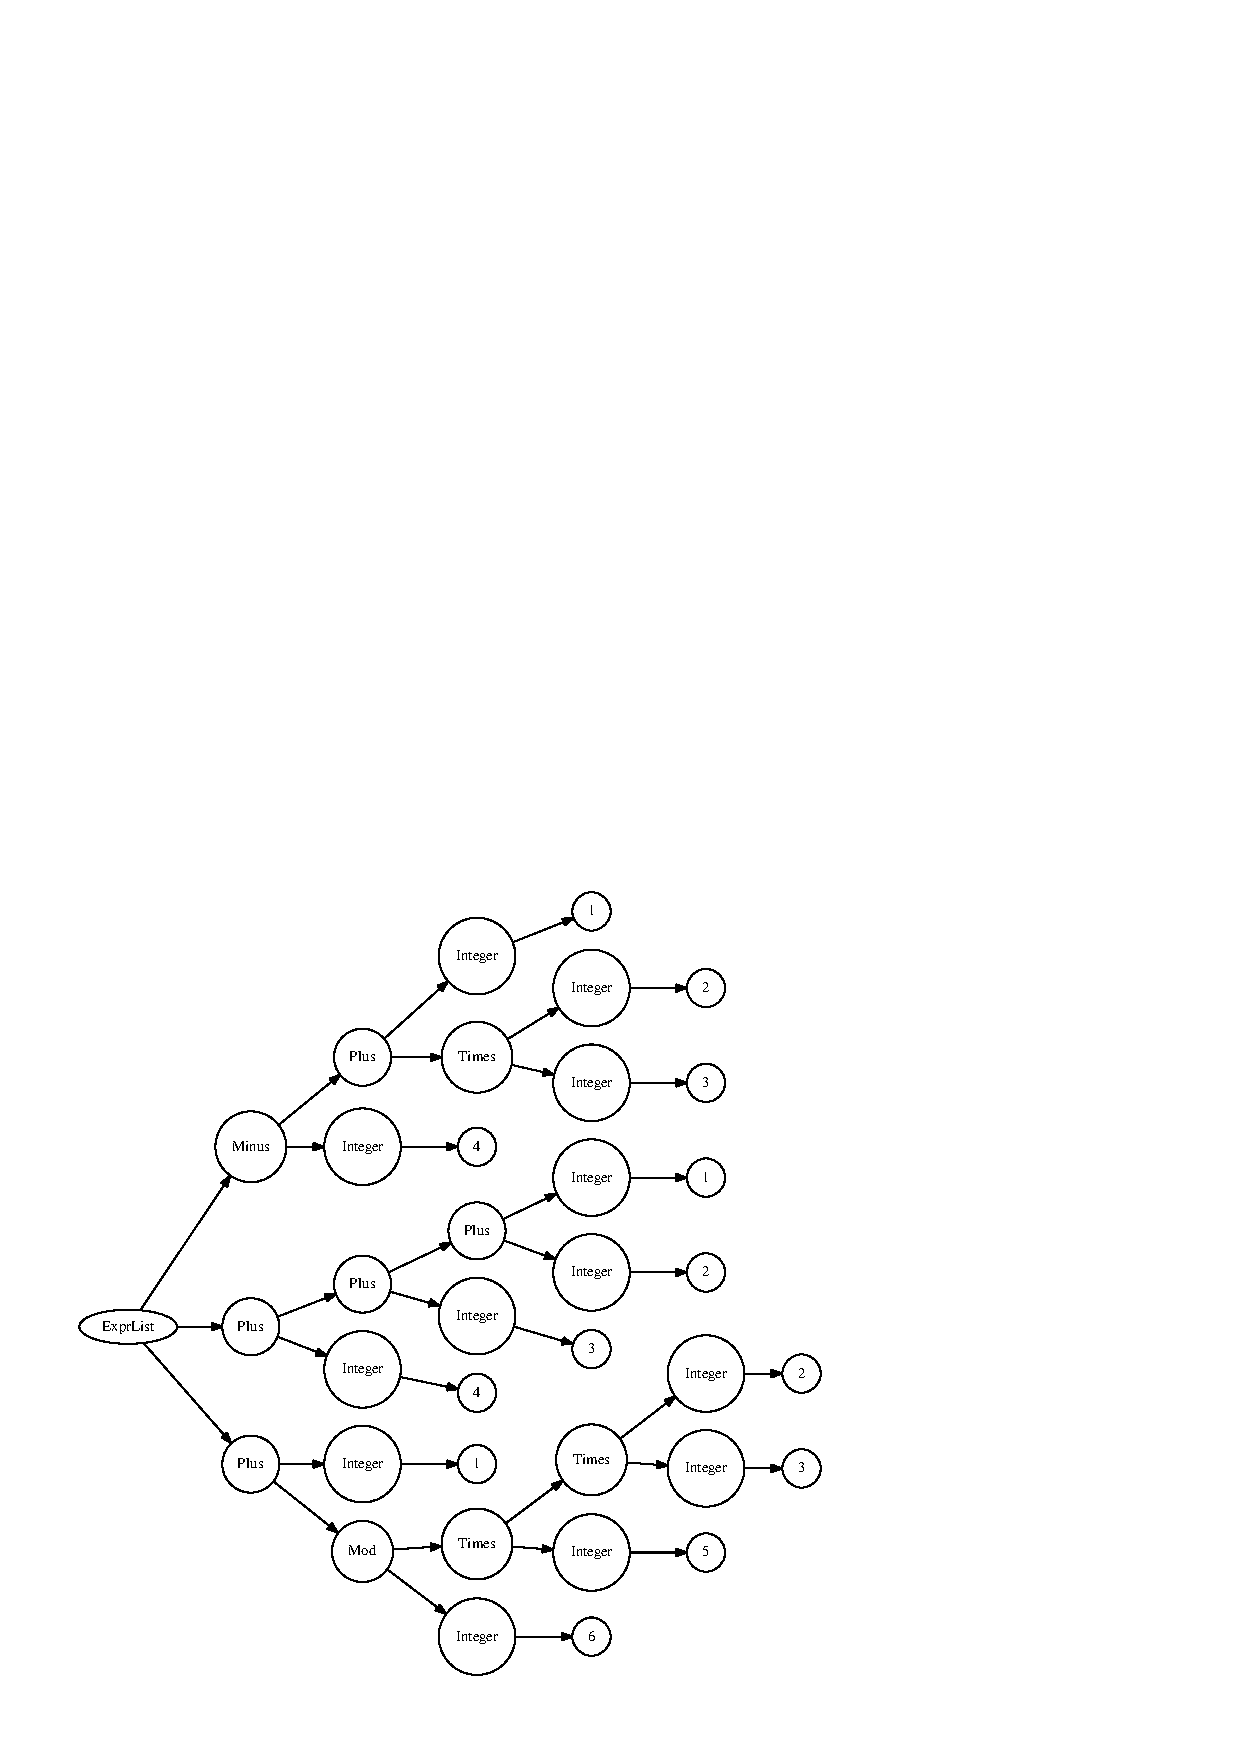
\includegraphics{arith_expr_tree.pdf}
	\caption{Arithexpr AST}
	\label{fig:arith_expr_tree}
\end{figure}

\subsection{Programming language grammar}
The programming language grammar and scanner.
The Scanner \mRefFigure{fig:example_interpreter_grammar_scanner} consists of the string literals for keywords and the definition of the syntax for a variable or function name, integers and decimals.
The Statements \mRefFigure{fig:example_interpreter_grammar_statements} describe the structure of the input file. It consists of multiple statement and definitions.
The Lists \mRefFigure{fig:example_interpreter_grammar_lists} describe how multiple arguments, expressions, definitions and statements are chained.
The Expressions \mRefFigure{fig:example_interpreter_grammar_expression} describe boolean and arithmetic expressions.
%\lstinputlisting[frame=single,numbers=left,basicstyle=\footnotesize ,breaklines=true]{interpreter_grammar_ast.g}
\begin{figure}[!ht]

\begin{Verbatim}[ frame         = lines, 
                  framesep      = 0.3cm, 
                  labelposition = bottomline,
                  numbers       = left,
                  numbersep     = -0.2cm,
                  xleftmargin   = 0.8cm,
                  xrightmargin  = 0.8cm,
                ]
  %%%
  FUNCTION    := function ;
  RETURN      := return ;
  IF          := if ;
  ELSE        := else ;
  WHILE       := while ;
  FOR         := for ;
  PRINT       := print ;
  QUIT        := exit ;
  STRING      := \"(?:\\.|[^\"])*\" ;
  WHITESPACE  := [ \t\v\r\s] ;
  SKIP        := {WHITESPACE}|\n|//[^\n]* ;
  INTEGER     := 0|[1-9][0-9]* ;
  DECIMAL     := 0\.[0-9]+|[1-9][0-9]*\.[0-9]+ ;
  ZID         := [a-zA-Z_][a-zA-Z0-9_]* ;  
  %%%
\end{Verbatim}
\caption{Example interpreter scanner}
\label{fig:example_interpreter_grammar_scanner}
\end{figure}
\begin{figure}[!ht]

\begin{Verbatim}[ frame         = lines, 
                  framesep      = 0.3cm, 
                  labelposition = bottomline,
                  numbers       = left,
                  numbersep     = -0.2cm,
                  xleftmargin   = 0.8cm,
                  xrightmargin  = 0.8cm,
                ]
  program 
   ::= dfnStmntList:d {: result := Program(d); :}
     ;
  dfnStmntList 
   ::= definition:d dfnStmntList:dl       {: result := [d] + dl; :}
     |  statement:stmts  dfnStmntList:dsl {: result := [stmts] + dsl; :}
     |                                    {: result := []; :}
     ;
  definition 
   ::= FUNCTION ZID:function_name '(' paramList:param_list ')' 
			'{' stmntList:statement_list '}'
       {: result := Function(function_name, param_list, statement_list);:}
     ;
  stmntList
   ::= statement:s stmntList:sl {: result := [s] + sl ; :}
     |  {: result := []; :}
     ;
  statement 
   ::= assignment:a ';'   {: result := Assign(a); :}    
     |  PRINT '(' printExprList:printexpr_list ')' ';'      
                          {: result := Print(printexpr_list); :}
     |  IF '(' boolExpr:b ')' '{' stmntList:st_list1 '}'    
                          {: result := If(b, st_list1); :}
     |  WHILE '(' boolExpr:b ')' '{' stmntList:st_list2 '}' 
                          {: result := While(b, st_list2); :}
     |  FOR '(' assignment:i_a ';' boolExpr:b ';' assignment:e_a ')' 
		    '{' stmntList:st_list3 '}' 
                          {: result := For(i_a, b, e_a, st_list3);  :}
     |  RETURN expr:e ';' {: result := Return(e); :}
     |  RETURN ';'        {: result := Return();  :}
     |  expr:e ';'        {: result := Expr(e);   :}      
     |  QUIT ';'          {: result := Exit();    :}
     ;
\end{Verbatim}
\caption{Example interpreter statements}
\label{fig:example_interpreter_grammar_statements}
\end{figure}
\begin{figure}[!ht]

\begin{Verbatim}[ frame         = lines, 
                  framesep      = 0.3cm, 
                  labelposition = bottomline,
                  numbers       = left,
                  numbersep     = -0.2cm,
                  xleftmargin   = 0.8cm,
                  xrightmargin  = 0.8cm,
                ]
  printExprList 
   ::= printExpr:p ',' nePrintExprList:np {: result := [p] + np ; :}
     |  printExpr:p                       {: result := [p]; :}
     |                                    {: result := [];  :}
     ;
  nePrintExprList
   ::= printExpr:p                         {: result := [p]; :}
     |  printExpr:p ',' nePrintExprList:np {: result := [p] + np ; :}
     ;
  printExpr 
   ::= STRING:string {: result := PrintString(string); :}
     |  expr:e       {: result := e; :}
     ;
  assignment 
   ::= ZID:id '=' expr:e {: result := Assign(id, e); :}
     ;
  paramList 
   ::= ZID:id ',' neIDList:nid {: result := [id] + nid ; :}
     |  ZID:id                 {: result := [id] ; :}
     |                         {: result := []; :}
     ;
  neIDList
   ::= ZID:id ',' neIDList:nid {: result := [id] + nid ; :}
     |  ZID:id                 {: result := [id] ; :}
     ;
  exprList
   ::= expr:e ',' neExprList:el {: result := [e] + el; :}
     |  expr:e                  {: result := [e]; :}
     |                          {: result := [];  :}
     ;
  neExprList
   ::= expr:e ',' neExprList:el {: result := [e] + el; :}
     |  expr:e                  {: result := [e]; :}
     ;
		\end{Verbatim}
\caption{Example interpreter Lists}
\label{fig:example_interpreter_grammar_lists}
\end{figure}
\begin{figure}[!ht]

\begin{Verbatim}[ frame         = lines, 
                  framesep      = 0.3cm, 
                  labelposition = bottomline,
                  numbers       = left,
                  numbersep     = -0.2cm,
                  xleftmargin   = 0.8cm,
                  xrightmargin  = 0.8cm,
                ]
  boolExpr 
   ::= expr:lhs '==' expr:rhs                {: result := Equation(lhs,rhs); :}
     |  expr:lhs '!=' expr:rhs               {: result := Inequation(lhs,rhs); :}
     |  disjunction:lhs '==' disjunction:rhs {: result := Equation(lhs,rhs); :}
     |  disjunction:lhs '!=' disjunction:rhs {: result := Inequation(lhs,rhs); :}
     |  expr:lhs '<=' expr:rhs               {: result := LessOrEqual(lhs,rhs);    :}
     |  expr:lhs '>=' expr:rhs               {: result := GreaterOrEqual(lhs,rhs); :}
     |  expr:lhs '<' expr:rhs                {: result := LessThan(lhs,rhs); :}
     |  expr:lhs '>' expr:rhs                {: result := GreaterThan(lhs,rhs); :}
     |  disjunction:d                        {: result := d; :}
     ;
  disjunction
   ::= disjunction:d '||' conjunction:c {: result := Disjunction(d,c); :}
     |  conjunction:c                   {: result := c; :}
     ;
  conjunction
   ::= conjunction:c '&&' boolFactor:f {:result := Conjunction(c,f); :}
     | boolFactor:f                    {: result := f; :}
     ;
  boolFactor
   ::= '(' boolExpr:be_par ')' {:  result := be_par; :}
     | '!' boolExpr:e          {: result := Negation(e); :}
     ;
  expr 
   ::= expr:e '+'   prod:p {: result := Sum(e,p); :} 
     |  expr:e '-'  prod:p {: result := Difference(e,p); :} 
     |  prod:p             {: result := p;     :}
     ;
  prod 
   ::= prod:p '*'  fact:f    {: result := Product(p,f); :}
     |  prod:p '\' fact:f    {: result := Quotient(p,f); :} 
     |  prod:p '%' fact:f    {: result := Mod(p,f); :} 
     |  fact:f               {: result := f;     :}
     ;
  fact 
   ::= '(' expr:e_par ')'            {: result := e_par;   :} 
     |  INTEGER:n                    {: result := Integer(eval(n));   :} 
     |  DECIMAL:d                    {: result := Decimal(eval(d)); :}
     |  ZID:id_1 '(' exprList:el ')' {: result := FunctionCall(id_1,el); :}
     |  ZID:id_2                     {: result := Variable(id_2); :}
     ;
		\end{Verbatim}
\caption{Example interpreter expressions}
\label{fig:example_interpreter_grammar_expression}
\end{figure}
A sample input program \mRefFigure{fig:example_interpreter_input} describes the recursive function factorial.
\begin{figure}[!ht]

\begin{Verbatim}[ frame         = lines, 
                  framesep      = 0.3cm, 
                  labelposition = bottomline,
                  numbers       = left,
                  numbersep     = -0.2cm,
                  xleftmargin   = 0.8cm,
                  xrightmargin  = 0.8cm,
                ]
  function factorial(n) {
      if (n == 0) {
         return 1;
      }
      return n * factorial(n - 1);
  }
  print("Calculation of factorial for i = 1 to 9");
  for (i = 0; i < 10; i = i + 1) {
      print(i, "! = ", factorial(i));
  }
  print();
		\end{Verbatim}
\caption{Example interpreter input}
\label{fig:example_interpreter_input}
\end{figure}
%\lstinputlisting[frame=single,numbers=left,basicstyle=\footnotesize ,breaklines=true]{factorial.sl}
The output AST \mRefFigure{fig:interpreter_tree} represents the syntactic structure of the factorial program. 
%\lstinputlisting[basicstyle=\footnotesize ,breaklines=true]{factorial_output.txt}


\begin{figure}
	\centering
		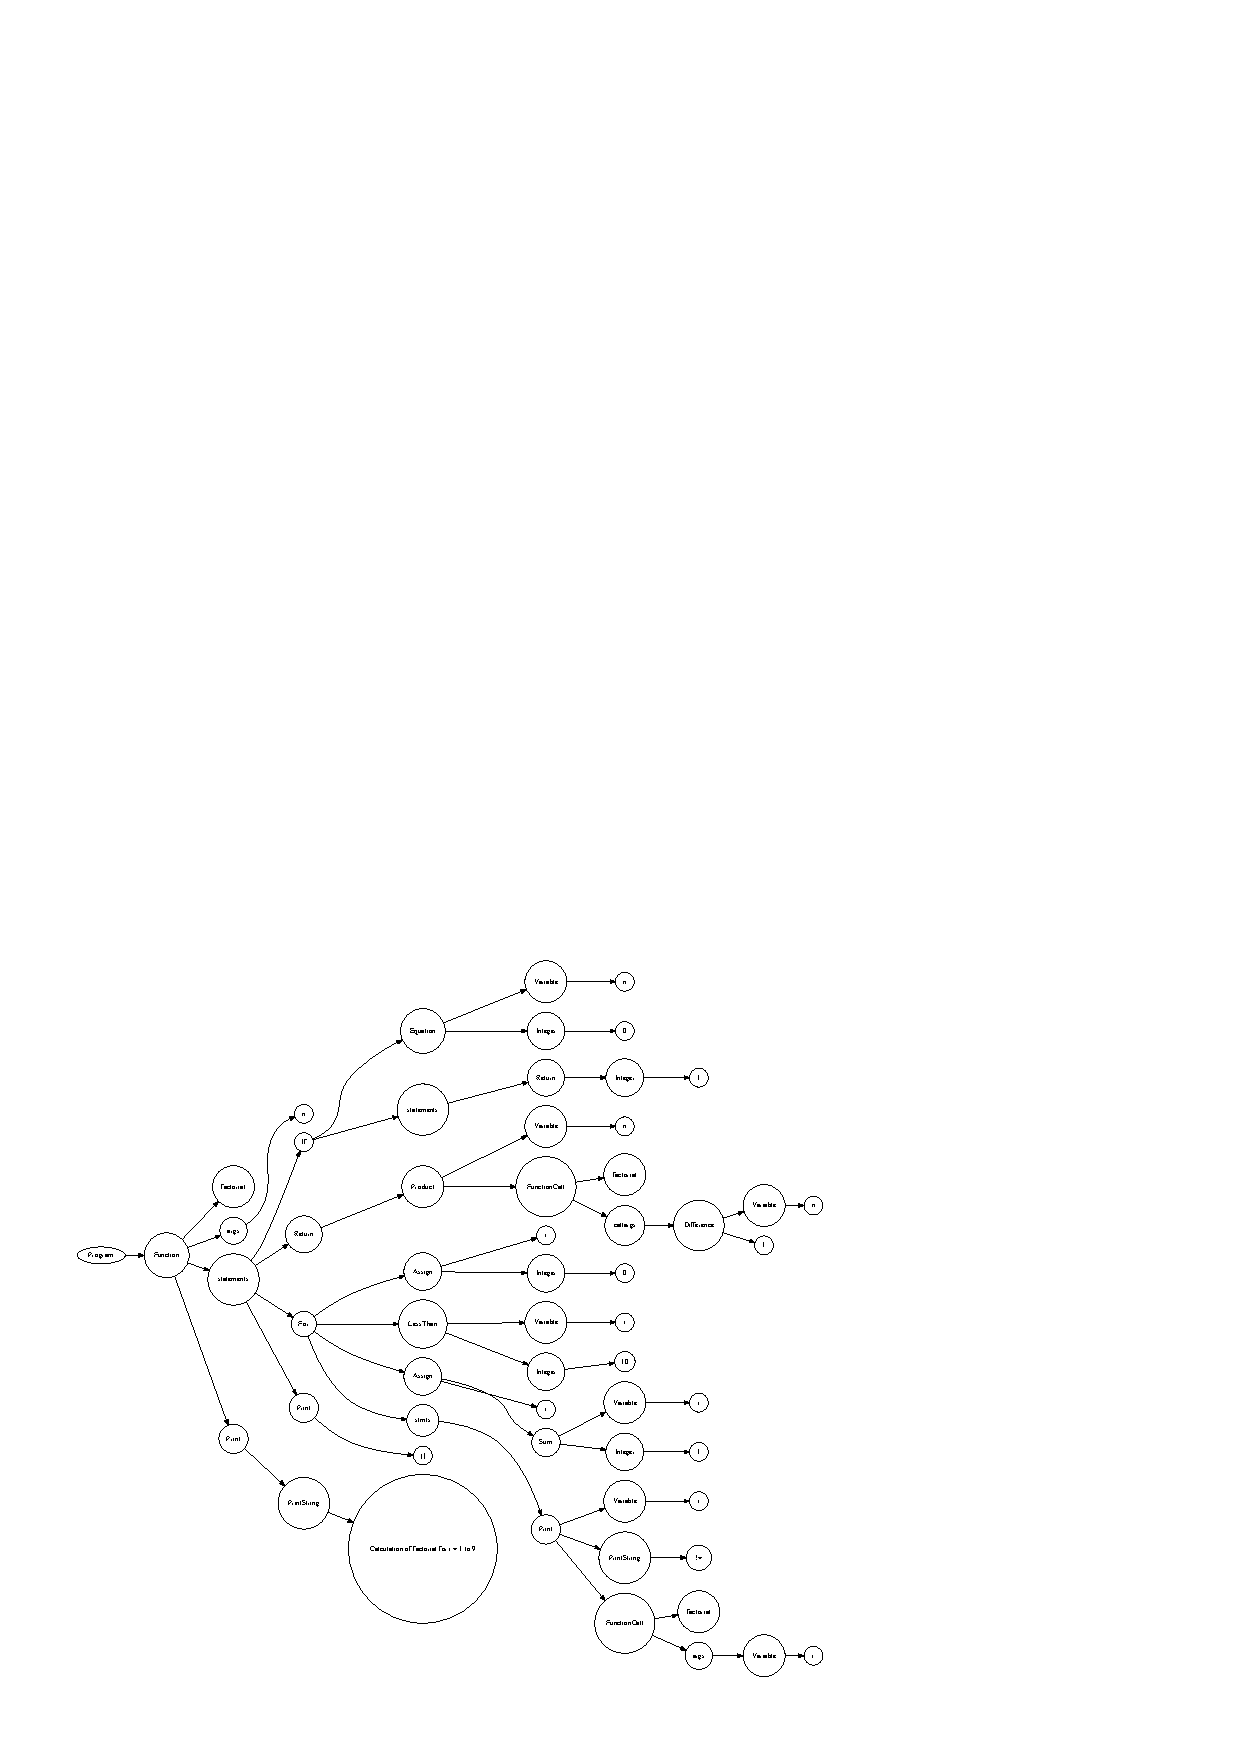
\includegraphics{interpreter_tree.pdf}
	\caption{Interpreter AST}
	\label{fig:interpreter_tree}
\end{figure}

